% !TeX program = pdfLaTeX
\documentclass[smallextended]{svjour3}       % onecolumn (second format)
%\documentclass[twocolumn]{svjour3}          % twocolumn
%
\smartqed  % flush right qed marks, e.g. at end of proof
%
\usepackage{amsmath}
\usepackage{graphicx}
\usepackage[utf8]{inputenc}

\usepackage[hyphens]{url} % not crucial - just used below for the URL
\usepackage{hyperref}

%
% \usepackage{mathptmx}      % use Times fonts if available on your TeX system
%
% insert here the call for the packages your document requires
%\usepackage{latexsym}
% etc.
%
% please place your own definitions here and don't use \def but
% \newcommand{}{}
%
% Insert the name of "your journal" with
% \journalname{myjournal}
%

%% load any required packages here


% Pandoc syntax highlighting
\usepackage{color}
\usepackage{fancyvrb}
\newcommand{\VerbBar}{|}
\newcommand{\VERB}{\Verb[commandchars=\\\{\}]}
\DefineVerbatimEnvironment{Highlighting}{Verbatim}{commandchars=\\\{\}}
% Add ',fontsize=\small' for more characters per line
\usepackage{framed}
\definecolor{shadecolor}{RGB}{248,248,248}
\newenvironment{Shaded}{\begin{snugshade}}{\end{snugshade}}
\newcommand{\AlertTok}[1]{\textcolor[rgb]{0.94,0.16,0.16}{#1}}
\newcommand{\AnnotationTok}[1]{\textcolor[rgb]{0.56,0.35,0.01}{\textbf{\textit{#1}}}}
\newcommand{\AttributeTok}[1]{\textcolor[rgb]{0.77,0.63,0.00}{#1}}
\newcommand{\BaseNTok}[1]{\textcolor[rgb]{0.00,0.00,0.81}{#1}}
\newcommand{\BuiltInTok}[1]{#1}
\newcommand{\CharTok}[1]{\textcolor[rgb]{0.31,0.60,0.02}{#1}}
\newcommand{\CommentTok}[1]{\textcolor[rgb]{0.56,0.35,0.01}{\textit{#1}}}
\newcommand{\CommentVarTok}[1]{\textcolor[rgb]{0.56,0.35,0.01}{\textbf{\textit{#1}}}}
\newcommand{\ConstantTok}[1]{\textcolor[rgb]{0.00,0.00,0.00}{#1}}
\newcommand{\ControlFlowTok}[1]{\textcolor[rgb]{0.13,0.29,0.53}{\textbf{#1}}}
\newcommand{\DataTypeTok}[1]{\textcolor[rgb]{0.13,0.29,0.53}{#1}}
\newcommand{\DecValTok}[1]{\textcolor[rgb]{0.00,0.00,0.81}{#1}}
\newcommand{\DocumentationTok}[1]{\textcolor[rgb]{0.56,0.35,0.01}{\textbf{\textit{#1}}}}
\newcommand{\ErrorTok}[1]{\textcolor[rgb]{0.64,0.00,0.00}{\textbf{#1}}}
\newcommand{\ExtensionTok}[1]{#1}
\newcommand{\FloatTok}[1]{\textcolor[rgb]{0.00,0.00,0.81}{#1}}
\newcommand{\FunctionTok}[1]{\textcolor[rgb]{0.00,0.00,0.00}{#1}}
\newcommand{\ImportTok}[1]{#1}
\newcommand{\InformationTok}[1]{\textcolor[rgb]{0.56,0.35,0.01}{\textbf{\textit{#1}}}}
\newcommand{\KeywordTok}[1]{\textcolor[rgb]{0.13,0.29,0.53}{\textbf{#1}}}
\newcommand{\NormalTok}[1]{#1}
\newcommand{\OperatorTok}[1]{\textcolor[rgb]{0.81,0.36,0.00}{\textbf{#1}}}
\newcommand{\OtherTok}[1]{\textcolor[rgb]{0.56,0.35,0.01}{#1}}
\newcommand{\PreprocessorTok}[1]{\textcolor[rgb]{0.56,0.35,0.01}{\textit{#1}}}
\newcommand{\RegionMarkerTok}[1]{#1}
\newcommand{\SpecialCharTok}[1]{\textcolor[rgb]{0.00,0.00,0.00}{#1}}
\newcommand{\SpecialStringTok}[1]{\textcolor[rgb]{0.31,0.60,0.02}{#1}}
\newcommand{\StringTok}[1]{\textcolor[rgb]{0.31,0.60,0.02}{#1}}
\newcommand{\VariableTok}[1]{\textcolor[rgb]{0.00,0.00,0.00}{#1}}
\newcommand{\VerbatimStringTok}[1]{\textcolor[rgb]{0.31,0.60,0.02}{#1}}
\newcommand{\WarningTok}[1]{\textcolor[rgb]{0.56,0.35,0.01}{\textbf{\textit{#1}}}}

% tightlist command for lists without linebreak
\providecommand{\tightlist}{%
  \setlength{\itemsep}{0pt}\setlength{\parskip}{0pt}}

% From pandoc table feature
\usepackage{longtable,booktabs,array}
\usepackage{calc} % for calculating minipage widths
% Correct order of tables after \paragraph or \subparagraph
\usepackage{etoolbox}
\makeatletter
\patchcmd\longtable{\par}{\if@noskipsec\mbox{}\fi\par}{}{}
\makeatother
% Allow footnotes in longtable head/foot
\IfFileExists{footnotehyper.sty}{\usepackage{footnotehyper}}{\usepackage{footnote}}
\makesavenoteenv{longtable}

% Pandoc citation processing
\newlength{\cslhangindent}
\setlength{\cslhangindent}{1.5em}
\newlength{\csllabelwidth}
\setlength{\csllabelwidth}{3em}
\newlength{\cslentryspacingunit} % times entry-spacing
\setlength{\cslentryspacingunit}{\parskip}
% for Pandoc 2.8 to 2.10.1
\newenvironment{cslreferences}%
  {}%
  {\par}
% For Pandoc 2.11+
\newenvironment{CSLReferences}[2] % #1 hanging-ident, #2 entry spacing
 {% don't indent paragraphs
  \setlength{\parindent}{0pt}
  % turn on hanging indent if param 1 is 1
  \ifodd #1
  \let\oldpar\par
  \def\par{\hangindent=\cslhangindent\oldpar}
  \fi
  % set entry spacing
  \setlength{\parskip}{#2\cslentryspacingunit}
 }%
 {}
\usepackage{calc}
\newcommand{\CSLBlock}[1]{#1\hfill\break}
\newcommand{\CSLLeftMargin}[1]{\parbox[t]{\csllabelwidth}{#1}}
\newcommand{\CSLRightInline}[1]{\parbox[t]{\linewidth - \csllabelwidth}{#1}\break}
\newcommand{\CSLIndent}[1]{\hspace{\cslhangindent}#1}

\usepackage{booktabs}
\begin{document}


\title{My Example Computed Manuscript }
 \subtitle{Created in Rmarkdown} 

    \titlerunning{Example computed manuscript}

\author{  Jeffrey M. Perkel \and  }


\institute{
        Jeffrey M. Perkel \at
     Springer Nature, 1 New York Plaza, New York, NY \\
     \email{\href{mailto:jeffrey.perkel@nature.com}{\nolinkurl{jeffrey.perkel@nature.com}}}  %  \\
%             \emph{Present address:} of F. Author  %  if needed
    \and
    }

\date{Received: date / Accepted: date}
% The correct dates will be entered by the editor


\maketitle

\begin{abstract}
A mock computed manuscript created in RStudio using \{Rmarkdown\}. The \{Bookdown\} and \{Rticles\} packages were used to output the text in Springer Nature's desired manuscript format.
\\
\keywords{
    }


\end{abstract}


\def\spacingset#1{\renewcommand{\baselinestretch}%
{#1}\small\normalsize} \spacingset{1}


\hypertarget{intro}{%
\section{Introduction}\label{intro}}

This is an R Markdown document. Markdown is a simple formatting syntax for authoring HTML, PDF, and MS Word documents. For more details on using R Markdown see \url{http://rmarkdown.rstudio.com}.

Here we'll add some references from Zotero (Perkel 2020): (Fisch et al. 2015; Argelaguet et al. 2021; Lê Cao et al. 2021).

Markdown documents can include inline equations written in \LaTeX, such as \(F = ma\). Here is an equation on its own line:

\[a^2 + b^2 = c^2\]

\hypertarget{results}{%
\section{Results}\label{results}}

\hypertarget{sec:1}{%
\subsection{Inline computation}\label{sec:1}}

The `killer feature' of computed manuscripts is their ability to compute and insert values and figures into the text rather than requiring authors to input them manually. That circumvents the possibility that the author will enter an incorrect number, or forget to update a figure or value should new data arise.

Imagine we are analyzing data from a clinical trial. We have grouped subjects in three bins and measured the concentration of some metabolite. (These data are simulated.)

Rather than analyzing those data and then copying the results into our manuscript, we can use the programming language \texttt{R} to do that in the manuscript itself. Simply enclose the code inside backticks, with the letter \texttt{r}: \texttt{\textasciigrave{}r\ \textless{}code\ to\ evaluate\textgreater{}\textasciigrave{}}. For instance, to calculate the circumference and area of a circle with radius \emph{r} = 10, you could write ``A = \texttt{\textasciigrave{}r\ pi\ *\ r\^{}2\textasciigrave{}}'' and ``C = \texttt{\textasciigrave{}r\ 2\ *\ pi\ *\ r\textasciigrave{}}. Those evaluate to''A = \textbf{314.159} and C = \textbf{62.832}''.

Returning to our dataset, we have \textbf{99} (simulated) subjects in our study. The average metabolite concentration is \textbf{185.36} (range: \textbf{78}-\textbf{298}). We have \textbf{32} subjects in Group 1, \textbf{43} subjects in Group 2, and \textbf{24} in Group 3. (The numbers in \textbf{bold face type} throughout this document are computed values.)

Now suppose we get another tranche of data. There are \textbf{60} subjects in this new dataset. Their average concentration is \textbf{185.13} (range: \textbf{77}-\textbf{299}).

Combining the two datasets, we have a total of \textbf{159} subjects (Table \ref{tab:show-table}). The revised average metabolite concentration is \textbf{185.28} (range: \textbf{77}-\textbf{299}). We now have \textbf{55} subjects in Group 1, \textbf{60} subjects in Group 2, and \textbf{44} in Group 3.

\hypertarget{sec:2}{%
\subsection{Data tables}\label{sec:2}}

\begin{table}

\caption{\label{tab:show-table}Final subject data}
\centering
\begin{tabular}[t]{llrlllrlllr}
\toprule
ID & Class & Conc & | & ID & Class & Conc & | & ID & Class & Conc\\
\midrule
ID\_1 & Group 2 & 153 & | & ID\_54 & Group 2 & 280 & | & ID\_107 & Group 3 & 170\\
ID\_2 & Group 1 & 224 & | & ID\_55 & Group 2 & 175 & | & ID\_108 & Group 3 & 78\\
ID\_3 & Group 2 & 127 & | & ID\_56 & Group 2 & 223 & | & ID\_109 & Group 1 & 129\\
ID\_4 & Group 2 & 194 & | & ID\_57 & Group 3 & 295 & | & ID\_110 & Group 1 & 137\\
ID\_5 & Group 1 & 251 & | & ID\_58 & Group 1 & 275 & | & ID\_111 & Group 3 & 217\\
\addlinespace
ID\_6 & Group 1 & 81 & | & ID\_59 & Group 2 & 120 & | & ID\_112 & Group 1 & 227\\
ID\_7 & Group 2 & 100 & | & ID\_60 & Group 1 & 78 & | & ID\_113 & Group 3 & 81\\
ID\_8 & Group 1 & 270 & | & ID\_61 & Group 3 & 78 & | & ID\_114 & Group 2 & 248\\
ID\_9 & Group 2 & 100 & | & ID\_62 & Group 3 & 140 & | & ID\_115 & Group 1 & 211\\
ID\_10 & Group 1 & 161 & | & ID\_63 & Group 3 & 294 & | & ID\_116 & Group 1 & 113\\
\addlinespace
ID\_11 & Group 3 & 158 & | & ID\_64 & Group 3 & 295 & | & ID\_117 & Group 1 & 216\\
ID\_12 & Group 3 & 118 & | & ID\_65 & Group 3 & 285 & | & ID\_118 & Group 3 & 91\\
ID\_13 & Group 2 & 143 & | & ID\_66 & Group 2 & 129 & | & ID\_119 & Group 3 & 258\\
ID\_14 & Group 2 & 258 & | & ID\_67 & Group 3 & 148 & | & ID\_120 & Group 2 & 85\\
ID\_15 & Group 3 & 224 & | & ID\_68 & Group 1 & 281 & | & ID\_121 & Group 3 & 181\\
\addlinespace
ID\_16 & Group 3 & 254 & | & ID\_69 & Group 3 & 295 & | & ID\_122 & Group 3 & 216\\
ID\_17 & Group 3 & 190 & | & ID\_70 & Group 2 & 111 & | & ID\_123 & Group 1 & 222\\
ID\_18 & Group 2 & 148 & | & ID\_71 & Group 2 & 132 & | & ID\_124 & Group 3 & 252\\
ID\_19 & Group 1 & 89 & | & ID\_72 & Group 2 & 261 & | & ID\_125 & Group 1 & 166\\
ID\_20 & Group 2 & 89 & | & ID\_73 & Group 1 & 122 & | & ID\_126 & Group 2 & 204\\
\addlinespace
ID\_21 & Group 3 & 253 & | & ID\_74 & Group 2 & 124 & | & ID\_127 & Group 2 & 243\\
ID\_22 & Group 3 & 231 & | & ID\_75 & Group 1 & 234 & | & ID\_128 & Group 3 & 198\\
ID\_23 & Group 1 & 112 & | & ID\_76 & Group 2 & 184 & | & ID\_129 & Group 1 & 119\\
ID\_24 & Group 2 & 277 & | & ID\_77 & Group 3 & 272 & | & ID\_130 & Group 1 & 198\\
ID\_25 & Group 2 & 197 & | & ID\_78 & Group 1 & 242 & | & ID\_131 & Group 3 & 151\\
\addlinespace
ID\_26 & Group 2 & 208 & | & ID\_79 & Group 2 & 277 & | & ID\_132 & Group 3 & 115\\
ID\_27 & Group 2 & 193 & | & ID\_80 & Group 3 & 236 & | & ID\_133 & Group 3 & 237\\
ID\_28 & Group 3 & 141 & | & ID\_81 & Group 1 & 101 & | & ID\_134 & Group 2 & 178\\
ID\_29 & Group 1 & 206 & | & ID\_82 & Group 3 & 218 & | & ID\_135 & Group 1 & 275\\
ID\_30 & Group 2 & 168 & | & ID\_83 & Group 2 & 130 & | & ID\_136 & Group 2 & 178\\
\addlinespace
ID\_31 & Group 2 & 298 & | & ID\_84 & Group 1 & 128 & | & ID\_137 & Group 3 & 267\\
ID\_32 & Group 1 & 144 & | & ID\_85 & Group 3 & 252 & | & ID\_138 & Group 1 & 95\\
ID\_33 & Group 2 & 241 & | & ID\_86 & Group 1 & 198 & | & ID\_139 & Group 1 & 108\\
ID\_34 & Group 2 & 221 & | & ID\_87 & Group 1 & 169 & | & ID\_140 & Group 2 & 77\\
ID\_35 & Group 1 & 112 & | & ID\_88 & Group 2 & 185 & | & ID\_141 & Group 1 & 299\\
\addlinespace
ID\_36 & Group 3 & 246 & | & ID\_89 & Group 1 & 216 & | & ID\_142 & Group 3 & 222\\
ID\_37 & Group 2 & 190 & | & ID\_90 & Group 2 & 185 & | & ID\_143 & Group 1 & 85\\
ID\_38 & Group 1 & 177 & | & ID\_91 & Group 2 & 97 & | & ID\_144 & Group 1 & 273\\
ID\_39 & Group 1 & 148 & | & ID\_92 & Group 2 & 165 & | & ID\_145 & Group 3 & 115\\
ID\_40 & Group 2 & 290 & | & ID\_93 & Group 3 & 89 & | & ID\_146 & Group 1 & 290\\
\addlinespace
ID\_41 & Group 2 & 151 & | & ID\_94 & Group 2 & 221 & | & ID\_147 & Group 2 & 269\\
ID\_42 & Group 2 & 159 & | & ID\_95 & Group 1 & 162 & | & ID\_148 & Group 2 & 97\\
ID\_43 & Group 2 & 113 & | & ID\_96 & Group 1 & 131 & | & ID\_149 & Group 1 & 229\\
ID\_44 & Group 1 & 249 & | & ID\_97 & Group 1 & 93 & | & ID\_150 & Group 3 & 176\\
ID\_45 & Group 1 & 124 & | & ID\_98 & Group 2 & 240 & | & ID\_151 & Group 2 & 164\\
\addlinespace
ID\_46 & Group 3 & 87 & | & ID\_99 & Group 2 & 86 & | & ID\_152 & Group 3 & 172\\
ID\_47 & Group 1 & 166 & | & ID\_100 & Group 2 & 219 & | & ID\_153 & Group 1 & 222\\
ID\_48 & Group 1 & 196 & | & ID\_101 & Group 2 & 243 & | & ID\_154 & Group 1 & 285\\
ID\_49 & Group 1 & 112 & | & ID\_102 & Group 2 & 213 & | & ID\_155 & Group 2 & 153\\
ID\_50 & Group 1 & 289 & | & ID\_103 & Group 1 & 177 & | & ID\_156 & Group 3 & 132\\
\addlinespace
ID\_51 & Group 2 & 161 & | & ID\_104 & Group 3 & 197 & | & ID\_157 & Group 2 & 156\\
ID\_52 & Group 3 & 270 & | & ID\_105 & Group 2 & 198 & | & ID\_158 & Group 1 & 260\\
ID\_53 & Group 2 & 237 & | & ID\_106 & Group 1 & 120 & | & ID\_159 & Group 2 & 201\\
\bottomrule
\end{tabular}
\end{table}

\hypertarget{sec:3}{%
\subsection{Plotting the data}\label{sec:3}}

We can also create and include figures during manuscript creation. Here we plot boxplots of our clinical trial data. The data are shown in Figure \ref{fig:plot-data}. Note that this figure number (as well as the table number above) is automatically generated.

\begin{figure}
\centering
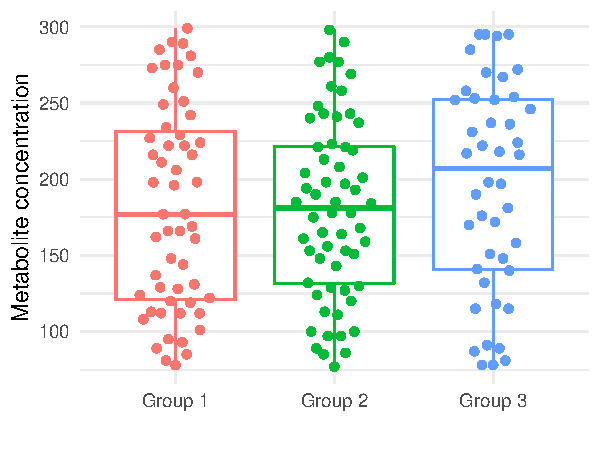
\includegraphics{SN_templates_files/figure-latex/plot-data-1.pdf}
\caption{\label{fig:plot-data}Metabolite concentration of clinical trial subjects}
\end{figure}

\hypertarget{code}{%
\section{Code}\label{code}}

The following code was used to load, merge, and plot the (simulated) clinical trial data:

\begin{Shaded}
\begin{Highlighting}[]
\CommentTok{\# load libraries}
\FunctionTok{library}\NormalTok{(tidyverse)}
\FunctionTok{library}\NormalTok{(ggbeeswarm)}
\FunctionTok{library}\NormalTok{(bookdown)}
\end{Highlighting}
\end{Shaded}

\begin{Shaded}
\begin{Highlighting}[]
\CommentTok{\# read in some initial data}
\NormalTok{df1 }\OtherTok{\textless{}{-}} \FunctionTok{read\_csv}\NormalTok{(}\StringTok{\textquotesingle{}example{-}data{-}1.csv\textquotesingle{}}\NormalTok{)}
\end{Highlighting}
\end{Shaded}

\begin{Shaded}
\begin{Highlighting}[]
\CommentTok{\# read new dataset}
\NormalTok{df2 }\OtherTok{\textless{}{-}} \FunctionTok{read\_csv}\NormalTok{(}\StringTok{\textquotesingle{}example{-}data{-}2.csv\textquotesingle{}}\NormalTok{)}
\end{Highlighting}
\end{Shaded}

\begin{Shaded}
\begin{Highlighting}[]
\CommentTok{\# merge datasets}
\NormalTok{final\_data }\OtherTok{\textless{}{-}} \FunctionTok{rbind}\NormalTok{(df1, df2)}
\end{Highlighting}
\end{Shaded}

\begin{Shaded}
\begin{Highlighting}[]
\CommentTok{\# plot the data}
\NormalTok{final\_data }\SpecialCharTok{\%\textgreater{}\%} 
  \FunctionTok{ggplot}\NormalTok{(}\FunctionTok{aes}\NormalTok{(}\AttributeTok{x =}\NormalTok{ class, }\AttributeTok{y =}\NormalTok{ conc, }\AttributeTok{color =}\NormalTok{ class)) }\SpecialCharTok{+}
  \FunctionTok{geom\_boxplot}\NormalTok{() }\SpecialCharTok{+}
\NormalTok{  ggbeeswarm}\SpecialCharTok{::}\FunctionTok{geom\_quasirandom}\NormalTok{(}\AttributeTok{width =} \FloatTok{0.25}\NormalTok{) }\SpecialCharTok{+} 
  \FunctionTok{xlab}\NormalTok{(}\StringTok{""}\NormalTok{) }\SpecialCharTok{+}
  \FunctionTok{ylab}\NormalTok{(}\StringTok{"Metabolite concentration"}\NormalTok{) }\SpecialCharTok{+} 
  \FunctionTok{theme\_minimal}\NormalTok{() }\SpecialCharTok{+}
  \FunctionTok{theme}\NormalTok{(}\AttributeTok{legend.position =} \StringTok{"none"}\NormalTok{)}
\end{Highlighting}
\end{Shaded}

\hypertarget{references}{%
\section*{References}\label{references}}
\addcontentsline{toc}{section}{References}

\hypertarget{refs}{}
\begin{CSLReferences}{1}{0}
\leavevmode\vadjust pre{\hypertarget{ref-argelaguet_computational_2021}{}}%
Argelaguet, Ricard, Anna S. E. Cuomo, Oliver Stegle, and John C. Marioni. 2021. {``Computational Principles and Challenges in Single-Cell Data Integration.''} \emph{Nature Biotechnology}, May, 1--14. \url{https://doi.org/10.1038/s41587-021-00895-7}.

\leavevmode\vadjust pre{\hypertarget{ref-fisch_omics_2015}{}}%
Fisch, K. M., T. Meissner, L. Gioia, J.-C. Ducom, T. M. Carland, S. Loguercio, and A. I. Su. 2015. {``Omics {Pipe}: A Community-Based Framework for Reproducible Multi-Omics Data Analysis.''} \emph{Bioinformatics} 31 (11): 1724--28. \url{https://doi.org/10.1093/bioinformatics/btv061}.

\leavevmode\vadjust pre{\hypertarget{ref-le_cao_community-wide_2021}{}}%
Lê Cao, Kim-Anh, Al J. Abadi, Emily F. Davis-Marcisak, Lauren Hsu, Arshi Arora, Alexis Coullomb, Atul Deshpande, et al. 2021. {``Community-Wide Hackathons to Identify Central Themes in Single-Cell Multi-Omics.''} \emph{Genome Biology} 22 (1): 220. \url{https://doi.org/10.1186/s13059-021-02433-9}.

\leavevmode\vadjust pre{\hypertarget{ref-perkel2020}{}}%
Perkel, Jeffrey M. 2020. {``Streamline Your Writing {\textemdash} and Collaborations {\textemdash} with These Reference Managers.''} \emph{Nature} 585 (7823): 149--50. \url{https://doi.org/10.1038/d41586-020-02491-2}.

\end{CSLReferences}


\bibliographystyle{spbasic}
\bibliography{bibliography.bib}


\end{document}
